\documentclass{article}
\usepackage[spanish]{babel}  
\usepackage[utf8]{inputenc} 
\usepackage{graphicx}

\title{\textbf{Propuesta de Proyecto:} \\Sistema de teleoperación basado en mediciones inerciales}
\author{\textit{Bernardo Aceituno-C. y Luis A. Pérez-B.}}
\date{}

\begin{document}

\begin{figure}
	\centering
	
\includegraphics[width=0.5\textwidth]{logo.png}
\end{figure}
\maketitle
\newpage
\section{Introducción}

Esta propuesta presenta una primera aproximación eal proyecto a realizar dentro de la asignatura EC3882. Se dispone de 12 semanas a partir del 12 de septiembre de 2016 para su realización. Se utilizan principalmente los implementos dispuestos en el Laboratorio C de la Universidad Simón Bolívar más ciertos adicionales adquiridos personalemente. El Prof. Calogero Bruscianelli se encargará de monitorear el buen desarrollo del proyecto. Se deben entregar, periodicamente, demostraciones que validen el cumplimiento del plan de trabajo.

\section{Proyecto}

\subsection{Justificación}

Hay situaciones en las cuales no existe la posibilidad de manipulación humana debido a la dificultad de acceso al medio o la necesidad de operación remota. Bajo estas situaciones surgen las alternativas de dispositivos teleoperados, controlados por el usuario en una estación remota. Estos sistemas acarrean beneficios desde el punto de vista de seguridad del usuario, evitando trabajos en ambientes inseguros.

Una plataforma de teleoperación típica consta de 3 componentes: estación de mando, sistema de comunicación y una o varias estaciones esclavas. Esta última consta de un robot móvil equipado con un manipulador en un entorno remoto. La estación de mando interactúa directamente con el usuario y es donde se encuentran la mayor cantidad de alternativas de diseño. El sistema de comunicación puede ser a través de redes de computadores o enlaces de RF, tomando en consideración elementos como latencia y consumo de energía.

De esta manera, se desea implementar un proyecto que sea una primera aproximación a las diferentes etapas del sistema teleoperación descrito. Se desea utilizar una interfaz gráfica como estación esclava, de tal manera de simular su comportamiento.

\subsection{Objetivos Específicos}
 
Al finalizar el trimestre se desea entregar un proyecto que cumpla con las siguientes caracteristicas:
 
\begin{enumerate}
    \item Estimar la posici\'on y orientaci\'on deseada para manipulador en base a las mediciones de los sensores.
    \item Implementar un filtro recursivo sobre las medidas de aceleraci\'on y orientaci\'on de forma embebida en el microcontrolador.
    \item Transmitir la informaci\'on estimada mediante un sistema de red local inalambrico.
    \item Enviar los datos leidos a una plataforma de  telemetr\'ia a distancia.
    \item Desarrollar un software de simulaci\'on para manipuladores sencillos dadas las medidas de posici\'on y orientaci\'on.
\end{enumerate}

\subsection{Etapas}

Para detallar el funcionamiento esperado del proyecto a desarollar se dividio a este en las siguientes etapas.

\begin{itemize}
	\item \textbf{Adquisición:} La primera etapa de interes se debe encargar de acondicionar las medidas de cada sensor para eliminar los efectos del ruido generado por el ambiente de trabajo en la medida usando filtrado anal\'ogico .
\end{itemize}

\begin{itemize}
	\item \textbf{Procesamiento:} Esta etapa debe estimar el desplazamiento del dispositivo y su orientaci\'on en base a las medidas realizadas y mediante el uso de un filtro recursivo (Kalman o complementario).
\end{itemize}

\begin{itemize}
	\item \textbf{Transmisión:} Esta etapa debe transmitir los datos obtenidos mediante hacia una red inalambrica local de forma que puedan ser leidos por un computador.
\end{itemize}

\begin{itemize}
	\item \textbf{Simulación:} Para verificar el funcionamiento del sistema de teleoperaci\'on se debe implementar un software que simule el funcionmaiento de este sobre un manipulador sencillo (un vehiculo aereo no tripulado o un brazo rob\'otico).
\end{itemize}

\subsection{Componentes}
A lo largo del proyecto se planea hacer uso de la siguiente lista de componentes:

\begin{enumerate}
	\item Amplificador de instrumentaci\'on INA126P
	\item Filtro Switched Capacitor TLC04CP
	\item Acelerometro Anal\'ogico Freescale MMA7260Q
	\item Gir\'oscopo digital L3G4200
	\item Microncontrolador Freescale MC9S08QE128
	\item Modulo WI-FI ESP8266
\end{enumerate}
\newpage
\subsection{Diagrama}

Las etapas presentadas en la secci\'on anterior se interconectan de la forma establecida en la figura \ref{fig:estructura_proyecto}.

\begin{figure}[h!]
    \centering
    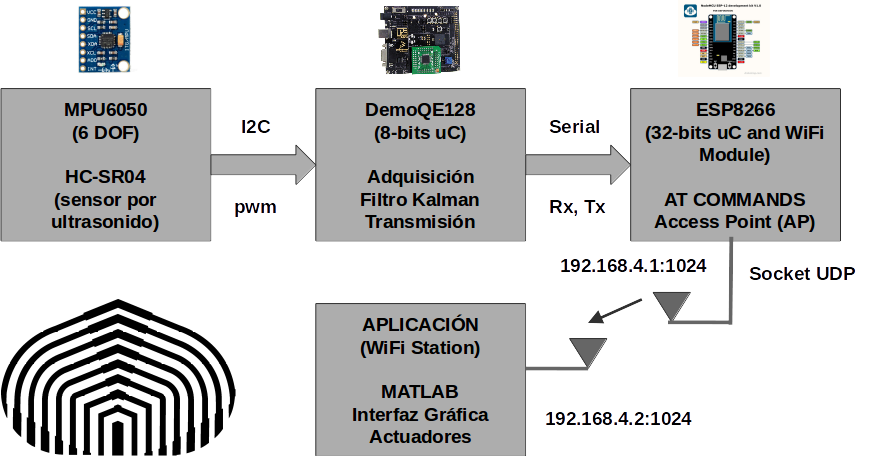
\includegraphics[width=1.0\textwidth]{diagrama1.png}
    \caption{Estructura del sistema}
    \label{fig:estructura_proyecto}
\end{figure}

Adicionalmente el sistema se puede representar como una maquina de estados como se muestra en la figure \ref{fig:maqn}.

\begin{figure}[h!]
	\centering
	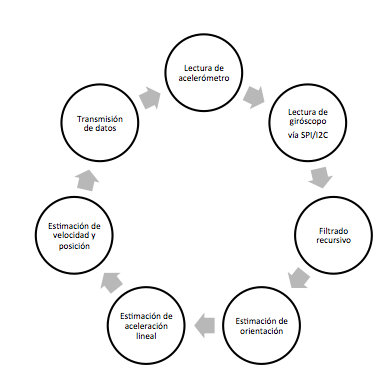
\includegraphics[width=0.5\textwidth]{diagrama2.png}
	\caption{Diagrama de estados del sistema}
	\label{fig:maqn}
\end{figure}

\section{Plan de Trabajo:} 
    Se presenta a continuación el plan de trabajo tentativo programado para ser desarrollado a lo largo del trimestre en curso:

\begin{table}[h!]
	\centering
	\caption{Plan de trabajo tentativo}
	\begin{tabular}{| c | p{10cm} |}
		\hline
		Semana 2& Revisi\'on bibliogr\'afica y familiarizaci\'on con el entorno de trabajo\\
		\hline
		Semana 3& Dise\~{n}o e Implementaci\'on de sistema de adquisici\'on\\
		\hline
		Semana 4& Pruebas en el funcionamiento del sistema de adquisici\'on y Dise\~{n}o del sistema de procesamiento\\
		\hline
		Semana 5& 
		\begin{enumerate} 
		    \item Implementaci\'on del sistema de procesamiento en el microcontrolador
		    \item Dise\~{n}o del sistema de transmisi\'on inalambrico
		\end{enumerate} \\
		\hline
		Semana 6&
		\begin{enumerate} 
		    \item Implementaci\'on del sistema de transmisi\'on inalambrico
		    \item Pruebas de funcionamiento del sistema de procesamiento
		    \item Dise\~{n}o del filtro recursivo embebido
		\end{enumerate}\\
		\hline
		Semana 7& 
		\begin{enumerate} 
		    \item Pruebas de funcionamiento del sistema de  transmisi\'on inalambrico y del sistema de procesamiento
		    \item Implementaci\'on del filtro recursivo embebido
		\end{enumerate}\\
		\hline
		Semana 8& 
		\begin{enumerate} 
		    \item Pruebas de funcionamiento del filtro recursivo embebido
		    \item Dise\~{n}o del software de simulaci\'on  y telemetr\'ia
		\end{enumerate}\\
		\hline
		Semana 9& 
		\begin{enumerate} 
		    \item Verificaci\'on de funcionamiento de la unidad de mediciones inerciales
		    \item Implementaci\'on del software de simulaci\'on  y telemetr\'ia
		\end{enumerate}\\
		\hline
		Semana 10& 
		\begin{enumerate} 
		    \item Verificaci\'on de funcionamiento del software de simulaci\'on y telemetr\'ia
		\end{enumerate}\\
		\hline
		Semana 11& Entrega del proyecto
		\\
		\hline
	\end{tabular}
\end{table}

\end{document}